\documentclass{article}
% V3-only template. V2 and its shared build inputs are left unchanged.
\makeatletter
\def\input@path{{../../docs/}}
\makeatother
\PassOptionsToPackage{numbers,compress}{natbib}
\usepackage[dblblindworkshop]{neurips_2026}
\workshoptitle{Foundation Models for the Brain and Body}
\usepackage[T1]{fontenc}
\usepackage{amsmath,amssymb}
\usepackage{newunicodechar}
\newunicodechar{−}{\ensuremath{-}}
\usepackage{graphicx}
\usepackage{float}
\usepackage{booktabs,longtable,array,calc}
\usepackage{microtype}
\usepackage{xcolor}
\usepackage{url}
\usepackage{hyperref}
\usepackage{placeins}
\usepackage{needspace}
\hypersetup{hidelinks,pdfauthor={},pdftitle={What Do Self-Supervised
Pose Representations Add Beyond Anatomy? Lessons for Body Foundation
Models from Gait Laterality}}
\setlength{\emergencystretch}{2em}
\setcounter{secnumdepth}{0}
\providecommand{\tightlist}{\setlength{\itemsep}{0pt}\setlength{\parskip}{0pt}}
\providecommand{\pandocbounded}[1]{#1}
% Optional display-only line breaks; PDF metadata retains the plain title.
\title{What Do Self-Supervised Pose Representations\\Add Beyond Anatomy?
Lessons for Body\\Foundation Models from Gait Laterality}
\author{Anonymous Author(s)}
\begin{document}
\maketitle
\begin{abstract}
Foundation models for the brain and body need features that preserve
movement information relevant to motor function. We develop a controlled
test using gait laterality: a measure derived from left--right
differences in landmark speed that reverses sign when the sides are
exchanged. We use 625 gait clips from 93 YouTube videos drawn from the
Gait Abnormality in Video Dataset (GAVD), a manually curated resource
for clinical gait analysis. Our quality-screened subset includes
annotations for normal gait and several neurological and muscular
conditions. We compare a compact pose encoder, trained by
self-supervised latent prediction, with its matched untrained version
while holding the body-landmark selection and prediction method fixed.
Test videos remain separate, and training is repeated from different
starting weights. Mirrored training examples improve feature consistency
under left--right exchange relative to training without them, but our
main prediction tests show no clear gain from either pretraining or
mirroring. A fixed prediction rule guarantees the expected sign change
even with features from an untrained encoder; with this rule held fixed,
pretraining without mirrored examples produces poorer predictions. The
study contributes an evaluation that distinguishes anatomically
consistent behavior from evidence that self-supervised pretraining
improves movement prediction. These experiments on a compact encoder
motivate testing whether larger body models gain predictive value beyond
their built-in anatomical structure. Connecting such comparisons to
independently measured gait is necessary before assigning physiological
meaning to the learned features.
\end{abstract}
\section{1. Introduction}\label{introduction}

A long-term goal of foundation models for the brain and body is to learn
representations that retain meaningful aspects of motor function. For
gait, this would mean that the model's \emph{latent space}---its
internal numerical description of movement---preserves useful
relationships between body parts and over time, while remaining reliable
across recording conditions. Clinical studies provide concrete examples
of what such representations might preserve: step length and the
duration of stance and swing are used to describe post-stroke gait
asymmetry, while the timing of successive left and right steps provides
a distinct measure of coordination
\citep{patterson2010symmetry, meijer2011coordination}.

Video-estimated body landmarks make these questions accessible without
laboratory motion capture. For the laterality evaluation, the encoder
receives 33 landmarks and predicts hidden features at 12 specified
locations: the shoulders, hips, knees, ankles, heels, and foot tips. The
shoulders and hips provide references for body alignment, while the
remaining locations describe lower-limb movement. Clinical gait research
motivates investigating this anatomical selection, but we have not
established that it is optimal or that its features measure neurological
impairment.

We use \emph{laterality}, defined here as a signed difference in
estimated movement between the left and right sides, to test what the
features preserve. The target averages speed contrasts from five
landmark pairs. Exchanging left and right must reverse its sign, giving
us a known response against which to test the model. We can evaluate
both prediction of the movement quantity and the features' response to
reflection, without assuming that either measures clinical impairment.

The central question is what learned pose features add beyond the body
structure and movement information already available to the model. We
compare a compact, pretrained S-JEPA-inspired encoder with its own
untrained starting weights, holding the architecture and anatomical
feature construction fixed \citep{abdelfattah2024sjepa}. Mirrored
training examples and a sign-constrained prediction rule let us examine
how anatomical knowledge affects the features and their predictions. An
exploratory condition-label classification check compares learned
features with simple pose summaries. Together, these comparisons connect
body-aware model design to evidence of predictive value, using baselines
suited to each task.

\section{2. Background and related
work}\label{background-and-related-work}

Joint-embedding predictive architectures learn by predicting hidden
feature representations. I-JEPA applies this approach to images, and
S-JEPA applies it to skeleton sequences
\citep{assran2023ijepa, abdelfattah2024sjepa}. Our laterality encoder
changes the architecture and training objective, so its results concern
the tested implementation and cohort. Related gait work, including
GaitForeMer, evaluates self-supervised representations against
gait-impairment severity \citep{endo2022gaitforemer}. The
coordinate-derived movement quantity used here offers a controlled test
before assigning clinical meaning to the representation.

Anatomical structure can enter a model through its layers, training
examples, or output rule. Group-equivariant networks and frame averaging
provide established ways to control responses to transformations
\citep{cohen2016gcnn, puny2022frame}. Reflection augmentation encourages
consistency through training, while the odd readout used here guarantees
a sign change algebraically. Clinical symmetry research motivates
examining the two sides separately \citep{patterson2010symmetry}, but
does not validate our particular speed contrast. The experimental
question is what these choices reveal about information accessible from
the learned features.

\section{3. Methods}\label{methods}

\subsection{3.1 Data and evaluation on unseen
videos}\label{data-and-evaluation-on-unseen-videos}

The Gait Abnormality in Video Dataset (GAVD) is a manually curated
resource for clinical gait analysis. Its creators sourced relevant
online videos, and clinicians screened and annotated the walking
sequences \citep{ranjan2025gavd}. We use pose extracted from a subset of
its YouTube videos with normal, Parkinson's, stroke, myopathic, or
cerebral-palsy annotations. A \emph{sequence} is a short annotated clip;
a \emph{source} is the original uploaded video. Quality and
target-computability checks retain 625 sequences from 93 sources out of
642 sequences with extracted pose. We form this eligible cohort before
assigning source folds. We take the dataset's condition categories as
given and make no independent clinical assessment of them.

We divide the 93 videos into five groups, approximately balancing
annotations. Each round trains on four groups and tests on the remaining
group, with every clip from a video kept together. These are the five
\emph{outer folds}: each video is test data once per seed. Five
\emph{seeds} vary the random initialization and training draws,
producing 25 trained encoders per training variant and 50 in total.
Grouping reduces shared-recording dependence
\citep{roberts2017crossvalidation}; reliable person identities are
unavailable, so the same individual may still appear in different
groups.

An exploratory condition-label classification check compares learned
features with simple pose summaries on 20 test videos. It uses a
separate encoder trained by introducing annotation categories in stages,
with one split and one initialization. Appendix B describes its methods
and overlapping cohort.

\subsection{3.2 Pretrain the laterality
encoder}\label{pretrain-the-laterality-encoder}

Each clip is represented by 33 pelvis-centered, scale-normalized
landmarks over 64 frames. Four consecutive XYZ observations at one
landmark form a patch, and a \emph{token} is the encoder's
representation of that patch. During training, up to 60\% of the
eligible patches at the 12 specified landmarks are hidden. Appendix A.1
gives the validity rules that decide which patches are eligible.

A four-layer, 96-dimensional encoder and a two-layer Transformer
predictor estimate the hidden features provided by a slowly updated
target encoder. The loss combines centered latent cross-entropy with a
two-view VICReg-style regularizer \citep{bardes2022vicreg}. Neither the
laterality target nor the annotation label enters this pretraining loss.

The variant without mirrored training clips never reflects a sample,
while the variant with mirrored training clips reflects each sample with
probability 0.5 before generating two training views. The two variants
share their initialization, source-draw schedules, and update counts, so
the reflection augmentation is the only intended difference between
them. Both receive 1,200 optimizer updates without early stopping.
Appendices A and C give the training details and pipeline overview.

\subsection{3.3 Define the left--right movement
quantity}\label{define-the-leftright-movement-quantity}

Reflection \(M\) negates the horizontal coordinate and exchanges
anatomical left/right landmark indices, including validity flags.
Applying it twice restores the input, so \(M^2=I\). For the shoulders,
knees, ankles, heels, and foot tips, we measure median left and right
speeds \(m_{L,k}\) and \(m_{R,k}\) on the same valid frame transitions:

\[
c_k=\frac{m_{L,k}-m_{R,k}}{m_{L,k}+m_{R,k}+10^{-8}},
\qquad y(X)=\frac{1}{5}\sum_{k=1}^{5}c_k.
\]

A positive pair contrast means the left landmark has the higher median
speed on that support. Every pair requires at least eight transitions
with both sides observed at both endpoints. Speeds use original
timestamps and uninterpolated normalized coordinates. Hips define pelvis
centering and are excluded from this target because their two centered
speed magnitudes coincide.

The construction gives \(y(MX)=-y(X)\) for any eligible clip, including
one with asymmetric movement. The target has mean -0.006 and standard
deviation 0.059. It is an estimated-coordinate motion index; its
relation to clinical gait measurements remains untested.

\subsection{3.4 Compare predictions with and without enforced sign
reversal}\label{compare-predictions-with-and-without-enforced-sign-reversal}

A \emph{readout} predicts laterality from encoder features using fitted
regression. Left/right mean tokens from five landmark pairs, pooled over
shared valid times, yield five differences and five sums. Concatenating
these gives a 960-value vector \(A(X)\) for pretrained and untrained
encoders.

The paper reports two readouts. The first predicts directly from
\(A(X)\), with no constraint on how the prediction responds to
reflection; this is the baseline against which pretraining is judged.
The second builds the sign reversal into the readout itself. Splitting
\(A(X)\) into the part that flips sign under reflection and the part
that does not,

\[
\Phi^-(X)=\frac{A(X)-A(MX)}{\sqrt{2}},
\qquad
\Phi^+(X)=\frac{A(X)+A(MX)}{\sqrt{2}},
\]

the odd part \(\Phi^-\) reverses sign under reflection while the even
part \(\Phi^+\) stays unchanged. A readout on the odd part with feature
centering and the intercept both disabled, \(h(X)=w^\top\Phi^-(X)\),
guarantees \(h(MX)=-h(X)\) for any encoder and any weights, whatever its
accuracy. This is what lets us ask whether correct sign behavior,
supplied by construction, carries any predictive benefit on its own.

Encoder weights stay fixed while separate regressions are fitted to
pretrained and untrained features. Four inner folds of outer-training
videos select each regression penalty; they tune only the readout,
although the encoder can already have seen these inputs during
pretraining. Appendix A.3 records two further readouts we examined but
do not report in the main comparison.

\subsection{3.5 Measure feature agreement and
uncertainty}\label{measure-feature-agreement-and-uncertainty}

We compare the encoder's features for a clip and its
left--right-mirrored copy after matching body landmarks---for example,
the mirrored left ankle with the original right ankle. The disagreement
score \(q\) compares these values directly, without fitted alignment.
Zero means complete agreement; larger scores mean more disagreement. A
feature that barely changes across clips will also agree closely with
its mirror, so a low score is consistent with either genuine symmetry or
near-constant features, and prediction accuracy is needed to tell them
apart. Appendix A gives the equation and validity checks.

For prediction, clips receive weights inverse to their source's clip
count, so each video has equal total weight. For each seed, we pool test
predictions from all five folds and calculate weighted sequence-level
\(R^2\), then average the five scores. An \(R^2\) of zero matches the
weighted-mean-target reference for the scored data; negative values
indicate larger squared error. This differs from averaging targets
within a video before scoring, or averaging predictions across seeds.

The 2,000 bootstrap samples redraw the 93 source videos with
replacement, carrying all their clips and seeds together. Both
conditions in each paired comparison use the same draws. The resulting
95\% intervals are pointwise and conditional on the fitted models and
fixed split. They omit uncertainty from retraining, alternative splits,
and choices made during development. Laterality estimates and intervals
use three decimal places to retain small differences; calculations and
relative reductions use unrounded values.

\section{4. Results}\label{results}

\subsection{4.1 Mirrored training improves feature
consistency}\label{mirrored-training-improves-feature-consistency}

Mirrored examples reduce feature disagreement by about 7\% compared with
training without them (reduction 0.008; 95\% interval {[}0.007,
0.010{]}). The video-balanced score is lower for each of the five
initializations. The features therefore agree more closely between
original and mirrored clips after matching left/right landmarks.
However, both pretrained variants still have greater average
disagreement than their matched untrained versions; the improvement is
between the two training variants.

\subsection{4.2 Prediction from learned and baseline
features}\label{prediction-from-learned-and-baseline-features}

Without enforced sign reversal, pretraining without mirrored examples
yields \(R^2=0.060\) (95\% interval {[}-0.025, 0.126{]}) on unseen
videos. Table 1 separates the effects of pretraining and mirrored
examples, including a comparison in which the sign-reversal rule is held
fixed.

\begin{longtable}[]{@{}
  >{\raggedright\arraybackslash}p{(\linewidth - 4\tabcolsep) * \real{0.4300}}
  >{\raggedleft\arraybackslash}p{(\linewidth - 4\tabcolsep) * \real{0.2900}}
  >{\raggedright\arraybackslash}p{(\linewidth - 4\tabcolsep) * \real{0.2800}}@{}}
\caption{Differences in laterality prediction; positive values indicate
improvement. Rows 1 and 3 compare the encoder pretrained without
mirrored clips with its matched untrained version; row 2 compares
training with versus without mirrored clips. Rows 1 and 2 do not enforce
sign reversal. Intervals are pointwise 95\% source-bootstrap intervals
conditional on fitted models (Appendix A.4).}\tabularnewline
\toprule\noalign{}
\begin{minipage}[b]{\linewidth}\raggedright
Question
\end{minipage} & \begin{minipage}[b]{\linewidth}\raggedleft
Difference in \(R^2\) (95\% interval)
\end{minipage} & \begin{minipage}[b]{\linewidth}\raggedright
What the result supports
\end{minipage} \\
\midrule\noalign{}
\endfirsthead
\toprule\noalign{}
\begin{minipage}[b]{\linewidth}\raggedright
Question
\end{minipage} & \begin{minipage}[b]{\linewidth}\raggedleft
Difference in \(R^2\) (95\% interval)
\end{minipage} & \begin{minipage}[b]{\linewidth}\raggedright
What the result supports
\end{minipage} \\
\midrule\noalign{}
\endhead
\bottomrule\noalign{}
\endlastfoot
Does pretraining improve prediction? & -0.018 {[}-0.039, 0.002{]} & No
clear improvement \\
Do mirrored training examples improve prediction? & +0.004 {[}-0.006,
0.013{]} & Improvement remains uncertain \\
With the sign rule fixed, does pretraining improve prediction? & -0.059
{[}-0.095, -0.017{]} & Pretrained encoder scores lower \\
\end{longtable}

The first two intervals include zero: neither pretraining nor mirroring
shows a clear prediction gain. The sign-reversal rule in the third
comparison holds for pretrained and untrained encoders, with numerical
checks passing for every seed. Under this rule, the encoder pretrained
without mirrored clips scores 0.059 lower in \(R^2\) than its matched
untrained version; the entire interval is below zero. Correct sign
behavior alone therefore cannot establish useful pretraining.

Simple input summaries provide another baseline for assessing learned
features. In the exploratory condition-label classification check, raw
pose summaries correctly classify 10 of 20 test videos, compared with 6
of 20 using learned features. This result supports retaining an
input-based comparison for that task, although the single-split design
and absence of a matched untrained encoder prevent attributing the
difference specifically to pretraining. Appendix B reports balanced
accuracy and a landmark-availability comparison.

\Needspace{10\baselineskip}

\section{5. Implications for physiologically meaningful
representations}\label{implications-for-physiologically-meaningful-representations}

The laterality comparisons isolate what pretraining adds, with the
anatomical inputs, feature construction, and form of the prediction rule
all held constant. On that footing we can compare features from
pretrained and matched untrained encoders, including the case where
correct left--right sign behavior is supplied by design rather than
learned. Mirrored examples improve feature agreement under reflection
without a clear prediction gain. The classification check asks whether
learned features beat simple summaries of the input; its result argues
for keeping a pose baseline, though it leaves open why the learned
features do worse.

A physiologically meaningful latent space remains a research objective.
Progress toward it would require testing whether features preserve
independently measured quantities such as step timing, joint motion, or
bilateral coordination across people and recording conditions. Our
signed speed contrast offers a controlled intermediate test, but cannot
substitute for those measurements. Adding a laterality-supervised loss
would also be a new experiment: the laterality encoder receives anatomy
through its inputs, target selection, and augmentation, without a
clinical or laterality label in its loss.

\section{6. Strengths, limitations, and responsible
use}\label{strengths-limitations-and-responsible-use}

Our laterality evaluation builds on GAVD's curated recordings with
matched training comparisons \citep{ranjan2025gavd}. Several safeguards
support it: test videos and all their clips are excluded from fitting
and tuning, which addresses dependence between clips from the same
recording \citep{roberts2017crossvalidation}; repeated training across
paired initializations reduces reliance on any single starting point;
and each video receives equal scoring weight, with the bootstrap
resampling whole videos to retain within-recording dependence (Section
3, Appendix A.4).

These safeguards support controlled laterality comparisons on unseen
source videos within GAVD, but they do not add independent recordings.
Person identities are unavailable, so performance on reliably separated
participants and an external cohort remains to be established. Estimated
pose and the speed index also require validation against measured gait
before clinical interpretation. The findings concern the tested encoder,
its linear prediction rules, and the specified reflection test, and the
classification encoder's training settings have not been independently
checked (Appendix B).

GAVD distributes its annotations under the MIT License, permitting
reuse, including academic research, subject to retaining the required
copyright and permission notices \citep{gavdMIT2026}. The source videos
are hosted separately; GAVD's access guidance specifies platform terms
and ethics and data-protection requirements for their use
\citep{gavdRepo2026}. Our study-specific ethics, video-use, and
derived-pose release reviews remain unresolved, so submission and data
release remain on hold. The experiments provide no basis for diagnosis,
surveillance, or clinical deployment.

\section{7. Conclusion}\label{conclusion}

Gait laterality offers a practical starting point for testing what
movement information a body representation preserves. Adding mirrored
clips improved feature consistency without a clear gain in predicting
left--right movement differences. The expected sign change could also be
built into the prediction rule with features from an untrained encoder,
so correct symmetry alone is no evidence that training helped. For body
foundation models, this makes predictive comparisons against matched
untrained features the test that judges what self-supervised training
adds.

\FloatBarrier\clearpage

\section{Appendix A. Laterality methods and
interpretation}\label{appendix-a.-laterality-methods-and-interpretation}

\subsection{A.1 Prepare the gait
clips}\label{a.1-prepare-the-gait-clips}

Quality checks and the requirement to calculate laterality retain 625
clips from 93 GAVD videos. The annotations comprise 270 normal, 39
Parkinson's, 75 stroke, 183 myopathic, and 58 cerebral-palsy clips. We
assign videos to the five evaluation groups after these checks, keeping
every clip from a video in the same group.

Coordinates follow the 33-landmark MediaPipe scheme
\citep{grishchenko2022blazepose}. An observed landmark must have finite
coordinates and a visibility score of at least 0.45. To calculate
laterality, both hips must be observed so coordinates can be centered at
their midpoint; body size is normalized using the median
three-dimensional shoulder and hip widths. We use original timestamps
and do not fill missing coordinates for this target. Each of the five
landmark pairs needs at least eight frame-to-frame intervals with both
sides observed at both ends, ensuring that left and right speeds use the
same observations.

For encoder inputs, gaps of up to four missing frames between valid
observations may be filled by interpolation, and clips are resized to 64
frames. We track which observations remain usable and set invalid
coordinates to zero. A four-frame patch is used only when all four
observations are marked valid. A clip must provide at least 50\% usable
observations across the 12 target landmarks and at least two complete
target-landmark patches after this preparation; filled gaps can
contribute to coverage. The advantage of this landmark selection over
alternatives has not been tested.

\subsection{A.2 Train with and without mirrored
clips}\label{a.2-train-with-and-without-mirrored-clips}

Both training conditions use a four-layer encoder with 96 feature values
per patch and a two-layer predictor, each with four attention heads. The
predictor estimates hidden features supplied by a slowly updated copy of
the encoder. The training objective is

\[
L_{\mathrm{pose}}=L_{\mathrm{latent\,CE}}+
0.05\left(25L_{\mathrm{invariance}}+
25L_{\mathrm{variance}}+L_{\mathrm{covariance}}\right).
\]

The first term measures how well the predicted features match their
targets. The remaining terms compare two slightly perturbed views of the
same clip: invariance encourages their features to agree, variance
discourages nearly constant features, and covariance discourages
redundant feature dimensions. The coefficient pattern 25, 25, and 1
follows VICReg \citep{bardes2022vicreg}; the variance and covariance
penalties are averaged across the two views. The multiplier 0.05 sets
their overall scale. These weights are fixed for both conditions, and
their suitability for gait has not been tested through a sensitivity
analysis.

Each encoder receives 1,200 AdamW updates with batches of 20 and an
initial learning rate of \(10^{-3}\). Each training epoch draws one clip
per training video, then samples additional videos uniformly to fill the
batches. The two conditions share starting weights, video draws, and
training length. Both use small rotations and translations; one also
mirrors clips with probability 0.5. Models are evaluated after the fixed
training period, without early stopping.

\subsection{A.3 Test prediction and feature
agreement}\label{a.3-test-prediction-and-feature-agreement}

For prediction, we compare each trained encoder with the same encoder at
its random starting weights. Both encoders remain fixed while separate
regressions are fitted to their features. Left/right features are
averaged over the same valid times, and all regressions use the same
feature width and tuning procedure. Four inner groups of training videos
select the regression penalty without using test videos. These groups
tune only the regression; their inputs can already have been used to
train the encoder.

The sign-reversal rule uses the difference between features from an
original clip and its mirrored copy (Section 3.4). The regression has no
intercept, and scaling preserves zero without subtracting a feature
mean. Together, these choices ensure that mirroring produces an
equal-magnitude prediction with the opposite sign, for either trained or
starting-weight features. We also examined two readouts not carried into
the main comparison: an odd-part readout that keeps its intercept, which
relaxes the exact sign guarantee, and an even-part readout on
\(\Phi^+\), which discards the sign-reversing information. Neither
changed the conclusions, and both are omitted from Table 1 to keep the
reported contrasts to the direct and sign-fixed readouts.

\Needspace{13\baselineskip}

Feature agreement is measured directly, without a prediction model. We
match left/right landmarks between the original and mirrored clips, then
divide their squared feature difference by their combined squared
magnitude:

\[
q(X)=
\frac{\lVert Z(MX)-SZ(X)\rVert_C^2}
{\lVert Z(MX)\rVert_C^2+\lVert SZ(X)\rVert_C^2}.
\]

\(Z(X)\) contains the encoder features across all 33 landmarks, and
\(MX\) is the mirrored clip. \(S\) exchanges left/right landmark
positions without changing feature channels; \(C\) selects positions
valid in both clips after landmark matching. The score requires at least
eight matched positions and a denominator that is not near zero. No
extra transformation is fitted to improve agreement. The score has no
units; zero means matching features, and larger values mean greater
disagreement. Features that change little between clips can also agree
closely, so the score must be considered alongside prediction accuracy.
It has no clinical calibration.

\FloatBarrier\Needspace{8\baselineskip}

\subsection{A.4 Checks and
uncertainty}\label{a.4-checks-and-uncertainty}

Every video receives equal total weight when fitting regressions and
calculating scores. For each initialization, we combine predictions from
all five held-out groups before calculating \(R^2\), then average the
five scores. Disagreement is calculated per clip before averaging with
equal video weight and then across initializations.

To estimate uncertainty, we resample the 93 videos 2,000 times, keeping
each video's clips and initializations together and using the same draw
for both conditions. The 95\% intervals apply to each comparison
separately and hold the fitted models fixed; they do not include
variation from retraining or different video splits.

We checked that test videos stayed out of fitting and tuning, paired
encoders shared their starting weights, and scores gave each video equal
weight. Recalculating the scores reproduced the reported values without
rerunning the models. The evaluation plan was finalized after
development and was not externally preregistered.

\Needspace{8\baselineskip}

\subsection{A.5 Reading Figure 1}\label{a.5-reading-figure-1}

Figure 1 shows the effects summarized in Section 4; this section
explains how to read the two panels and adds one point the main text
does not. Panel B is the feature-disagreement comparison and panel A the
prediction comparison, both as differences with pointwise 95\%
intervals.

One feature of panel B is worth drawing out. The reduction from mirrored
clips is measured between the two training variants, yet both variants
sit above their untrained references, so those reference comparisons
fall below zero. Mirroring therefore helps relative to training without
it, while neither trained encoder agrees with its mirror as closely as
its own random starting weights do. Panel A carries the prediction story
of Table 1: the first two contrasts straddle zero, and the sign-fixed
contrast is the one that turns clearly negative once the prediction rule
is fixed the same way for both encoders.

\begin{figure}
\centering
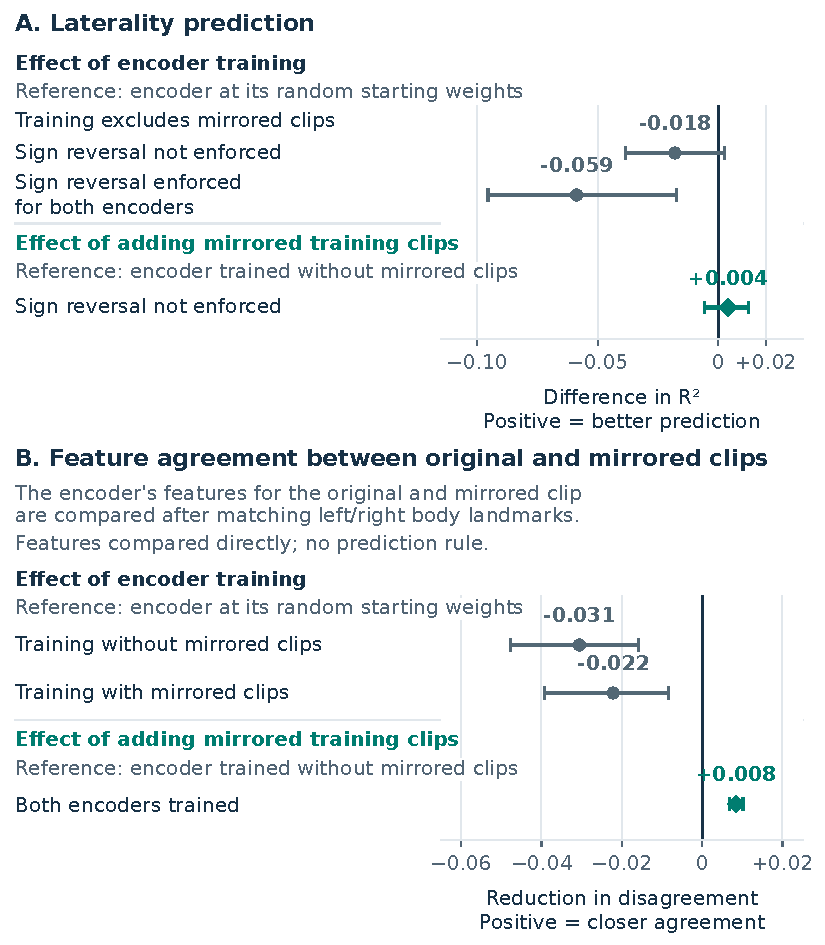
\includegraphics[width=1\linewidth,height=\textheight,keepaspectratio,alt={Effects of encoder training and mirrored training clips. Encoder training refers to pretraining the model that converts pose into features. In each panel, the first group compares the trained encoder with the same encoder at its random starting weights. In A, a regression is fitted separately to each encoder's features while encoder weights remain fixed. The first two rows in A exclude mirrored training clips and differ in whether sign reversal is enforced for both encoders. Enforcing it requires equal-magnitude, opposite-sign predictions when left and right are exchanged. The second group in each panel compares encoders trained with versus without mirrored clips. A shows prediction R\^{}2 minus reference R\^{}2; B shows reference disagreement minus the tested encoder's disagreement. B compares features directly after matching left/right landmarks, without a prediction rule. Positive values favor the tested condition; zero means no difference. Points average video-balanced paired estimates over five initializations, each covering five held-out video groups. Bars show pointwise 95\% intervals from resampling whole videos while keeping fitted models fixed. Intervals crossing zero include possible gains and losses.}]{figures/submission_laterality_effects_v3.pdf}
\caption{Effects of encoder training and mirrored training clips.
Encoder training refers to pretraining the model that converts pose into
features. In each panel, the first group compares the trained encoder
with the same encoder at its random starting weights. In A, a regression
is fitted separately to each encoder's features while encoder weights
remain fixed. The first two rows in A exclude mirrored training clips
and differ in whether sign reversal is enforced for both encoders.
Enforcing it requires equal-magnitude, opposite-sign predictions when
left and right are exchanged. The second group in each panel compares
encoders trained with versus without mirrored clips. A shows prediction
\(R^2\) minus reference \(R^2\); B shows reference disagreement minus
the tested encoder's disagreement. B compares features directly after
matching left/right landmarks, without a prediction rule. Positive
values favor the tested condition; zero means no difference. Points
average video-balanced paired estimates over five initializations, each
covering five held-out video groups. Bars show pointwise 95\% intervals
from resampling whole videos while keeping fitted models fixed.
Intervals crossing zero include possible gains and losses.}
\end{figure}

\FloatBarrier\clearpage

\section{Appendix B. Predicting gait-condition
labels}\label{appendix-b.-predicting-gait-condition-labels}

This exploratory comparison asks whether learned pose features help
distinguish GAVD's five annotated gait categories. It uses 639
quality-screened clips from 97 YouTube videos, divided into 59 training,
18 validation, and 20 test videos. All clips from a video stay together,
with assignments fixed before pose-quality checks. The recordings
overlap those in the laterality evaluation and do not provide an
independent replication.

The encoder is trained to predict hidden pose features while
discouraging nearly constant or redundant features. Training begins with
normal-annotated clips, then adds the Parkinson's, stroke, myopathic,
and cerebral-palsy categories in that order, retaining the earlier
categories. Annotations determine this schedule, but are not prediction
targets during encoder training. The benefit of the ordering was not
tested.

We compare summaries of landmark positions and frame-to-frame movement
with summaries of the encoder's features. A third input records how
often landmarks are available, without their coordinates. This checks
whether missing or poorly detected landmarks carry information about the
annotation labels.

A logistic-regression classifier is fitted separately for each input
type, with feature scaling and greater weight for less common
categories. Encoder weights stay fixed during classifier fitting.
Validation videos guide encoder selection and classifier tuning; the
final classifiers use all 77 training and validation videos. Test videos
remain excluded from these steps.

\begin{longtable}[]{@{}
  >{\raggedright\arraybackslash}p{(\linewidth - 4\tabcolsep) * \real{0.4600}}
  >{\raggedleft\arraybackslash}p{(\linewidth - 4\tabcolsep) * \real{0.2900}}
  >{\raggedleft\arraybackslash}p{(\linewidth - 4\tabcolsep) * \real{0.2500}}@{}}
\caption{Prediction of dataset annotations on 20 held-out videos.
Balanced accuracy is the fraction classified correctly within each
category, averaged equally across the five categories. Higher values
indicate better performance; scores are rounded to two
decimals.}\tabularnewline
\toprule\noalign{}
\begin{minipage}[b]{\linewidth}\raggedright
Features used
\end{minipage} & \begin{minipage}[b]{\linewidth}\raggedleft
Videos correctly classified
\end{minipage} & \begin{minipage}[b]{\linewidth}\raggedleft
Balanced accuracy
\end{minipage} \\
\midrule\noalign{}
\endfirsthead
\toprule\noalign{}
\begin{minipage}[b]{\linewidth}\raggedright
Features used
\end{minipage} & \begin{minipage}[b]{\linewidth}\raggedleft
Videos correctly classified
\end{minipage} & \begin{minipage}[b]{\linewidth}\raggedleft
Balanced accuracy
\end{minipage} \\
\midrule\noalign{}
\endhead
\bottomrule\noalign{}
\endlastfoot
Pose and movement summaries & 10/20 & 0.44 \\
Learned pose features & 6/20 & 0.26 \\
Landmark availability only & 6/20 & 0.25 \\
\end{longtable}

Simple pose summaries perform best here, although all three methods
misclassify the three stroke-annotated test videos. This supports
retaining pose summaries as a baseline. The evidence comes from one
split and one training initialization, with no comparison against the
same encoder at its random starting weights, so the difference cannot be
attributed specifically to pretraining.

Fitting and testing also combine clips differently: fitting uses average
features per video, while testing averages the class probabilities
predicted for individual clips. This difference can affect the results,
as can low-confidence landmark estimates entering the encoder. The exact
encoder-training settings have not been independently verified.

\FloatBarrier\clearpage

\section{Appendix C. From video to laterality
evaluation}\label{appendix-c.-from-video-to-laterality-evaluation}

A fixed MediaPipe model processes GAVD's annotated walker crops,
producing image-normalized horizontal and vertical coordinates,
estimated relative depth, and visibility scores. These estimates are not
calibrated motion-capture measurements. Laterality calculation and
encoder-input preparation follow separate paths (Appendix A.1).

Our S-JEPA adaptation \citep{abdelfattah2024sjepa} selects valid patches
uniformly within the 12 specified landmarks and hides their content
while retaining their positions. The target encoder follows a running
average of the trainable encoder's weights without receiving gradient
updates. For evaluation, we freeze this target encoder and a copy with
its saved random starting weights. Each supplies features to a
separately fitted laterality regression; the pretraining predictor is
not used for this step. Additional regularization uses two unmasked,
perturbed views through the trainable encoder (Appendix A.2).

\begin{figure}[H]
\centering
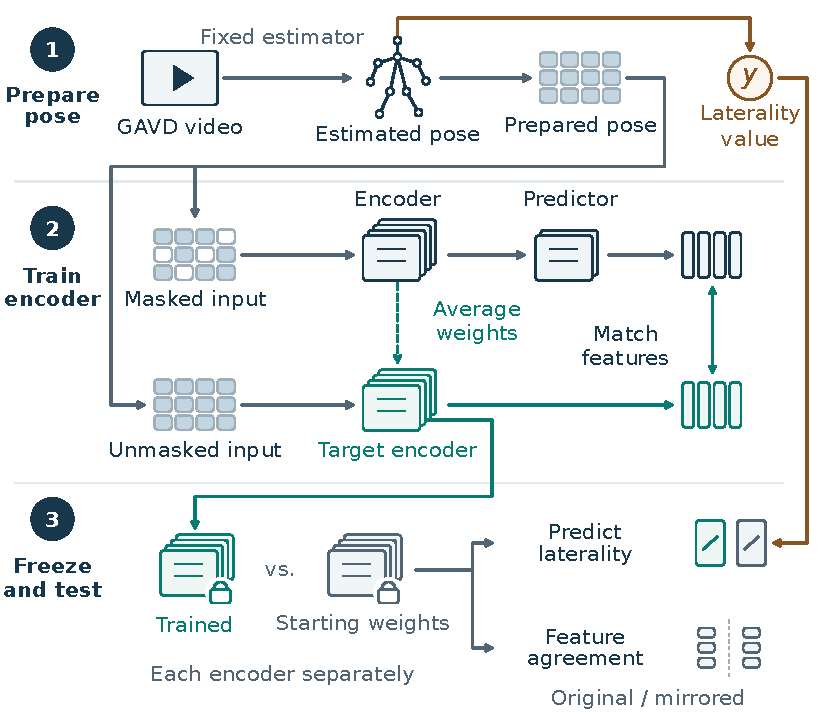
\includegraphics[width=1\linewidth,height=\textheight,keepaspectratio,alt={Workflow for training with and without mirrored clips. The gold path carries the laterality value to prediction fitting and scoring, outside encoder pretraining. Each frozen encoder's regression is fitted separately on training videos. Held-out videos test laterality prediction and feature agreement between original and mirrored clips, with left/right landmarks matched for the feature comparison.}]{figures/submission_pipeline_v3.pdf}
\caption{Workflow for training with and without mirrored clips. The gold
path carries the laterality value to prediction fitting and scoring,
outside encoder pretraining. Each frozen encoder's regression is fitted
separately on training videos. Held-out videos test laterality
prediction and feature agreement between original and mirrored clips,
with left/right landmarks matched for the feature comparison.}
\end{figure}
\clearpage
{\small
\bibliographystyle{plainnat}
\bibliography{../../docs/references,bbfm2026_paper_V3_references}
}
\end{document}
